\begin{frameExample}{The Simplex Algorithm}{}
  % EXAMPLE  2.9-3 Gupta ebook
  \begin{onlyenv}<1>
Solve the example~\ref{example:2-9-3_Gupta-ebook} with the simplex algorithm
  \begin{columns}
    \column{0.4\textwidth}
    \[ \max Z = 2x_1 + x_2 \]
      
    {\centering
      subject to

      \sysdelim..%
      \sysalign{r,r}%
      \systeme[x_1x_2]%
      {
        x_1 + 2x_2  \leq 10,
        x_1 + x_2  \leq 6,
        x_1 - x_2  \leq 2,
        x_1 - 2x_2  \leq 1
      }

      \vspace{5mm}
      $x_1, x_2  \geq 0$
      \par}
    \column{0.6\textwidth}
    \[ \max Z = 2x_1 + x_2 \]

    {\centering
      s.t.%
      
        \sysdelim..%
        \sysalign{r,r}%
        \systeme[x_1x_2s_1s_2s_3s_4]%
        {%
          x_1 + 2x_2 + s_1  = 10,
          x_1 + x_2 + s_2 = 6,
          x_1  - x_2  + s_3 = 2,
          x_1  - 2x_2  + s_4 = 1
        } % systeme

      \vspace{5mm}
      $x_1, x_2, s_1, s_2, s_3, s_4  \geq 0$
      \par}
  \end{columns}
  \end{onlyenv}


\begin{onlyenv}<2>
  Tabla Simplex Inicial
  
  {\centering
\begin{tabular}{rc|rr|rrrr|r}
  &$\max$  & $x_1$ & $x_2$ & $s_1$ &$ s_2$ & $s_3$ & $s_4$ &  \\
  \toprule
  $\mathbf{C_b}$ & \textbf{basis} & 2 & 1 & 0 & 0 & 0 & 0 & RHS \\
  \midrule
0 & $s_1$ & 1 & 2 & 1 & 0 & 0 & 0 & 10 \\
0 & $s_2$ & 1 & 1 & 0 & 1 & 0 & 0 & 6 \\
0 & $s_3$ & 1 & -1 & 0 & 0 & 1 & 0 & 2 \\
  0 & $s_4$ & 1 & -2 & 0 & 0 & 0 & 1 & 1\\
  \bottomrule
\end{tabular}
  \par}
\end{onlyenv}

\begin{onlyenv}<3>  
  {\centering
      \begin{tabular}{rc|rrrrrr|rr}
  &  $\max$ & $x_1$ & $x_2$ & $s_1$ &$ s_2$ & $s_3$ & $s_4$ & & \\
  \toprule
$\mathbf{C_b}$ & \textbf{basis} & 2 & 1 & 0 & 0 & 0 & 0 & RHS & ratios \\
  \midrule
%%%% 1
  0 & $s_1$ & 1 & 2 & 1 & 0 & 0 & 0 & 10 & 10 \\
0 & $s_2$ & 1 & 1 & 0 & 1 & 0 & 0 & 6 & 6 \\
0 & $s_3$ & 1 & -1 & 0 & 0 & 1 & 0 & 2 & 2 \\
  0 & $s_4$ & \cellcolor{yellow}1 & -2 & 0 & 0 & 0 & 1 & 1 & 1 \\
  \midrule
Iter& $Z_j$ & 0 & 0 & 0 & 0 & 0 & 0 & 0 &  \\
 1& $c_j - Z_j$ & 2 & 1 & 0 & 0 & 0 & 0 &  & 
   %%%%%%%%
\end{tabular}
  \par}
\end{onlyenv}

\begin{onlyenv}<4>
    {\centering
      \begin{tabular}{rc|rrrrrr|rr}
  &  $\max$ & $x_1$ & $x_2$ & $s_1$ &$ s_2$ & $s_3$ & $s_4$ & & \\
  \toprule
$\mathbf{C_b}$ & \textbf{basis} & 2 & 1 & 0 & 0 & 0 & 0 & RHS & ratios \\
  \midrule
%%%%%%%%%% 2
        0 & $s_1$ & 0 & 4 & 1 & 0 & 0 & -1 & 9 &  \\
0 & $s_2$ & 0 & 3 & 0 & 1 & 0 & -1 & 5 &  \\
0 & $s_3$ & 0 & 1 & 0 & 0 & 1 & -1 & 1 &  \\
        2 & $x_1$ & \cellcolor{yellow}1 & -2 & 0 & 0 & 0 & 1 & 1 &  \\
        \midrule
Iter & $Z_j$ & 2 & -4 & 0 & 0 & 0 & 2 & 2 &  \\
1 & $c_j - Z_j$ & 0 & 5 & 0 & 0 & 0 & -2 &  & 
        %%%%%%%%
\end{tabular}
  \par}
\end{onlyenv}

\begin{onlyenv}<5>
    {\centering
      \begin{tabular}{rc|rrrrrr|rr}
  &  $\max$ & $x_1$ & $x_2$ & $s_1$ &$ s_2$ & $s_3$ & $s_4$ & & \\
  \toprule
$\mathbf{C_b}$ & \textbf{basis} & 2 & 1 & 0 & 0 & 0 & 0 & RHS & ratios \\
  \midrule
%%%%%%%% 3
0 & $s_1$ & 0 & 4 & 1 & 0 & 0 & -1 & 9 & \nicefrac{9}{4} \\
0 & $s_2$ & 0 & 3 & 0 & 1 & 0 & -1 & 5 &  \nicefrac{5}{3} \\
0 & $s_3$ & 0 & \cellcolor{yellow}1 & 0 & 0 & 1 & -1 & 1 & 1 \\
        2 & $x_1$ & 1 & -2 & 0 & 0 & 0 & 1 & 1 & \nicefrac{-1}{2}\\
        \midrule
Iter & $Z_j$ & 2 & -4 & 0 & 0 & 0 & 2 & 2 &  \\
2 & $c_j - Z_j$ & 0 & 5 & 0 & 0 & 0 & -2 &  & 
          %%%%%%%%
\end{tabular}
  \par}
\end{onlyenv}

\begin{onlyenv}<6>
    {\centering
      \begin{tabular}{rc|rrrrrr|rr}
  &  $\max$ & $x_1$ & $x_2$ & $s_1$ &$ s_2$ & $s_3$ & $s_4$ & & \\
  \toprule
$\mathbf{C_b}$ & \textbf{basis} & 2 & 1 & 0 & 0 & 0 & 0 & RHS & ratios \\
  \midrule
%%%%%% 4
0 & $s_1$ & 0 & 0 & 1 & 0 & -4 & 3 & 5 &  \\
0 & $s_2$ & 0 & 0 & 0 & 1 & -3 & 2 & 2 &  \\
1 & $x_2$ & 0 & \cellcolor{yellow}1 & 0 & 0 & 1 & -1 & 1 &  \\
        2 & $x_1$ & 1 & 0 & 0 & 0 & 2 & -1 & 3 &  \\
        \midrule
Iter & $Z_j$ & 2 & 1 & 0 & 0 & 5 & -3 & 7 &  \\
2 & $c_j - Z_j$ & 0 & 0 & 0 & 0 & -5 & 3 &  & 
  %%%%%%%%
\end{tabular}
  \par}
\end{onlyenv}

\begin{onlyenv}<7>
      {\centering
      \begin{tabular}{rc|rrrrrr|rr}
  &  $\max$ & $x_1$ & $x_2$ & $s_1$ &$ s_2$ & $s_3$ & $s_4$ & & \\
  \toprule
$\mathbf{C_b}$ & \textbf{basis} & 2 & 1 & 0 & 0 & 0 & 0 & RHS & ratios \\
  \midrule
  %%%%%%%% 5
0 & $s_1$ & 0 & 0 & 1 & 0 & -4 & 3 & 5 & \nicefrac{5}{3} \\
0 & $s_2$ & 0 & 0 & 0 & 1 & -3 & \cellcolor{yellow}2 & 2 & 1 \\
1 & $x_2$ & 0 & 1 & 0 & 0 & 1 & -1 & 1 & -1 \\
        2 & $x_1$ & 1 & 0 & 0 & 0 & 2 & -1 & 3 & -3 \\
        \midrule
Iter & $Z_j$ & 2 & 1 & 0 & 0 & 5 & -3 & 7 &  \\
3 & $c_j - Z_j$ & 0 & 0 & 0 & 0 & -5 & 3 &  & 
            %%%%%%
\end{tabular}
  \par}
\end{onlyenv}

\begin{onlyenv}<8>
      {\centering
      \begin{tabular}{rc|rrrrrr|rr}
  &  $\max$ & $x_1$ & $x_2$ & $s_1$ &$ s_2$ & $s_3$ & $s_4$ & & \\
  \toprule
$\mathbf{C_b}$ & \textbf{basis} & 2 & 1 & 0 & 0 & 0 & 0 & RHS & ratios \\
  \midrule
%%%%%%%% 6
0 & $s_1$ & 0 & 0 & 1 & -1.5 & 0.5 & 0 & 2 &  \\
0 & $s_4$ & 0 & 0 & 0 & 0.5 & -1.5 & \cellcolor{yellow}1 & 1 &  \\
1 & $x_2$ & 0 & 1 & 0 & 0.5 & -0.5 & 0 & 2 &  \\
        2 & $x_1$ & 1 & 0 & 0 & 0.5 & 0.5 & 0 & 4 &  \\
        \midrule
Iter & $Z_j$ & 2 & 1 & 0 & 1.5 & 0.5 & 0 & 10 &  \\
3 & $c_j - Z_j$ & 0 & 0 & 0 & -1.5 & -0.5 & 0 &\textbf{END}  & 
          %%%%%%%%
\end{tabular}
  \par}
\end{onlyenv}


\begin{onlyenv}<9>
  {centering
  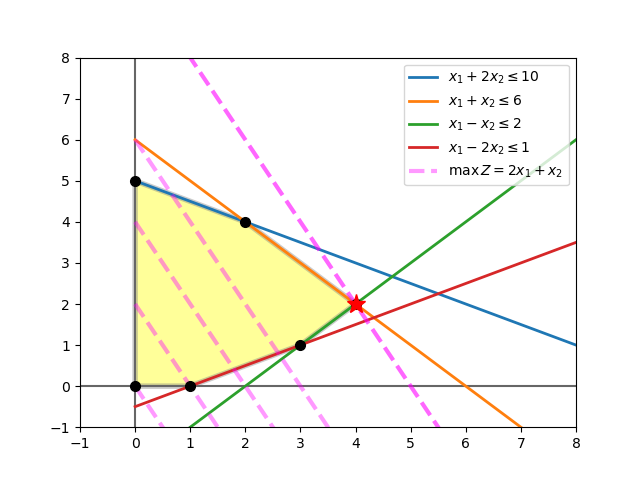
\includegraphics[scale=0.5]{fig_example-simplex03.png}
  \par}
\end{onlyenv}
\end{frameExample}

%%% Local Variables:
%%% mode: latex
%%% TeX-master: "slides"
%%% End:
